\documentclass[11pt,a4paper]{article}
\usepackage[margin=2.2cm]{geometry}
\usepackage{graphicx,booktabs,url,amsmath}
\usepackage[hidelinks]{hyperref}
\graphicspath{{../../fullsim_analysis/results/bench/2026-10-22/}}
\title{Noise of the Citiroc front end: how it is measured, and what the bench shows}
\author{CaLibrated AUtomatic Document Entity (CLAUDE), supervised by J. J. G\'omez-Cadenas}
\date{23 October 2026}
\begin{document}
\maketitle

\section{Purpose}

The electronic noise of the readout enters the energy resolution, the width of the
single-photoelectron peaks used for the calibration, and the value stored by channels that
receive little light. The simulation describes it with a simple model, which has to be checked
and, where it fails, replaced by one that reproduces the measurements. This note describes how
the noise of the system ---the SiPMs, the Citiroc and the A5202 board that carries it--- is
measured, then applies the method to the measurements as they arrive, records where they
disagree with the model, the hypotheses that could explain the disagreement and the
measurements that would distinguish them. It is a working record: new measurements are added
as cases, and the last section states what is stable enough to be passed to the model of the
simulation.

\section{The readout chain}

Each A5202 board reads 64 SiPMs with two Citiroc chips of 32 channels, and biases them with its
own HV module through a common line. In each channel of the Citiroc the SiPM signal is
amplified by two preamplifiers in parallel, the high gain and the low gain, and each path is
shaped by a slow shaper (one differentiation and two integrations, CR-RC$^2$, with a peaking
time $t_p$ that can be set to 25, 50 or 87.5~ns). In the peak stretch mode a peak detector
follows the maximum of the shaped signal between the trigger and the hold, which comes
\texttt{HoldDelay} after the trigger, and the value it holds is digitised by a 13-bit ADC. The
32 channels of a chip are held and read at the same trigger.

\section{How the noise is measured}
\label{sec:method}

\subsection{Pedestal runs}

The noise is measured in pedestal runs: the SiPMs are connected and biased 1--2~V below
breakdown, so that no avalanche contributes while their capacitance stays at the input of the
preamplifiers, and the board is triggered periodically, uncorrelated with any signal. Each run
gives, for every channel and event, the value stored in both gains. Changing the shaping
between runs, with \texttt{HoldDelay} = 0, gives the dependence of the noise on the peaking
time, which separates its components (Section~\ref{sec:observables}); changing
\texttt{HoldDelay} at a fixed shaping changes the window over which the peak detector takes the
maximum, which tells how fast the noise varies. A last run repeating the first checks the
stability of the pedestals.

\subsection{Separating the common mode}
\label{sec:cm}

Part of the noise may be shared by all the channels of a chip, and it can be separated because
they are read at the same trigger. For one chip and one run, with $x_i(e)$ the value of
channel $i$ in event $e$:
\begin{enumerate}
\item \textbf{Deviations from the pedestal.}
  \begin{equation*}
  d_i(e) = x_i(e) - \operatorname{median}_e\, x_i .
  \end{equation*}
\item \textbf{Jumps of the whole chip.} The number of channels far from their pedestal,
  \begin{equation*}
  N(e) = \#\{\, i : |d_i(e)| > 60 \text{ counts} \,\},
  \end{equation*}
  with 60 counts about five times the rms, flags events in which the whole chip jumps, a fault
  rather than noise. Events with $N(e) \ge 10$ are counted and set aside.
\item \textbf{Common mode.} The common mode of an event is the mean of the deviations,
  \begin{equation*}
  \mathrm{CM}(e) = \frac{1}{32}\sum_{i=1}^{32} d_i(e) .
  \end{equation*}
\item \textbf{Coupling of each channel.} The separation assumes that every channel receives the
  same common mode. This is checked with the slope of each channel against it,
  \begin{equation*}
  b_i = \frac{\mathrm{cov}_e(d_i, \mathrm{CM})}{\mathrm{var}_e\, \mathrm{CM}} ,
  \end{equation*}
  which is 1 for a channel that takes the full common mode. A channel with a slope far from 1
  is coupled differently from the others, and the slope says how.
\item \textbf{Total, coherent and incoherent noise.}
  \begin{align*}
  \sigma_\mathrm{tot} &= \operatorname{median}_i\, \mathrm{rms}_e\, d_i , \\
  \sigma_\mathrm{inc} &= \operatorname{median}_i\, \mathrm{rms}_e \big(d_i - \mathrm{CM}\big)\,\sqrt{32/31} , \\
  \sigma_\mathrm{coh}^2 &= \mathrm{var}_e\, \mathrm{CM} - \sigma_\mathrm{inc}^2/32 .
  \end{align*}
  The two corrections come from the mean itself: subtracting it removes from each channel 1/32
  of its own noise, and it keeps $1/\sqrt{32}$ of the incoherent noise of the channels, which
  is not common. The check is $\sigma_\mathrm{tot}^2 = \sigma_\mathrm{coh}^2 +
  \sigma_\mathrm{inc}^2$.
\item \textbf{Correlation between chips.} The correlation coefficient of the common modes of
  two chips, over the events both read, says whether the common mode is that of the chip, of
  the board, or of the whole system.
\end{enumerate}

\subsection{What each observable tells}
\label{sec:observables}

\begin{itemize}
\item \textbf{Noise against shaping.} After a CR-RC shaper, white series noise (the noise of
  the preamplifier input, which grows with the capacitance at the input) scales as
  $t_p^{-1/2}$, white parallel noise (leakage current, bias resistors) as $t_p^{+1/2}$, and a
  $1/f$ noise does not depend on $t_p$. The dependence of each part, coherent and incoherent,
  on the shaping points to its components.
\item \textbf{Pedestal against the window.} In the peak stretch the stored value is the maximum
  of the noise over the window, so the pedestal rises and narrows as \texttt{HoldDelay} grows.
  How fast it does so depends on how many independent fluctuations fit in the window, that is
  on the correlation time of the noise; an ideal peak detector is assumed.
\item \textbf{Low gain against high gain.} The two paths share the input and have their own
  preamplifiers: a noise entering before them is scaled by the ratio of their gains, a noise
  of their own is not.
\item \textbf{Coherent noise, its correlation and the slopes.} Where the common noise enters:
  a chip, a board or the system, and through which part of the input.
\end{itemize}

\subsection{From ADC counts to photoelectrons}

All the quantities above are in ADC counts. Expressing them in photoelectrons, which is what
the simulation and the calibration need, takes the gain of each path in counts per
photoelectron, at each shaping and overvoltage. It is measured with the SiPMs above breakdown,
from the spacing of the single-photoelectron peaks of the dark counts (hold-delay scan,
calibration with the periodic trigger).

\section{The noise model of the simulation}
\label{sec:model}

The simulation makes three assumptions:
\begin{enumerate}
\item \textbf{Series white noise.} After the slow shaper the noise rms scales as $t_p^{-1/2}$.
  It is set to 0.1~photoelectron (pe) in the high gain at 87.5~ns and 3~V of overvoltage,
  hence 0.06~pe at 5~V; at 50 and 25~ns it is 1.32 and 1.87 times larger.
\item \textbf{Same noise in both gains.} The low gain has the same rms in ADC counts as the
  high gain at the same shaping.
\item \textbf{Independent channels.} The noise of each channel is independent of that of the
  others.
\end{enumerate}
With an ideal peak detector, white noise shaped at 25~ns gives a pedestal that rises by 1.7
times the rms of a single sample at a \texttt{HoldDelay} of 96~ns and 2.2 at 296~ns, with the
width reduced to 0.6 and 0.5 of that rms: a window of 96~ns already contains several
independent fluctuations.

\section{Case: pedestal runs of 22 October 2026}
\label{sec:case1}

\subsection{The data}

Five A5202 boards (320 channels), the SiPMs biased at 36.5~V, below breakdown, a periodic
trigger every 1~ms, about 10\,000 events per run. Three runs at \texttt{HoldDelay} = 0 change
the shaping of the high gain (25, 50, 87.5~ns); five more at 25~ns change \texttt{HoldDelay}
from 96 to 496~ns; a last run repeats the first. The low gain is shaped at 87.5~ns in all runs.
Channels 0--31 of two boards are not read (a readout problem under investigation), which
leaves eight chips of 32 channels. The gain was not measured, so the results are in ADC counts.

\subsection{The steps on one chip}

The method of Section~\ref{sec:cm} is illustrated on one chip that works normally (board 2,
channels 32--63, run 26, high gain at 25~ns).

Besides the fluctuations of each channel, the map of the deviations $d_i$ shows vertical
stripes, events in which most channels are above or below their pedestal together
(Figure~\ref{fig:stepA}): this is the common mode.

\begin{figure}[h]
\centering
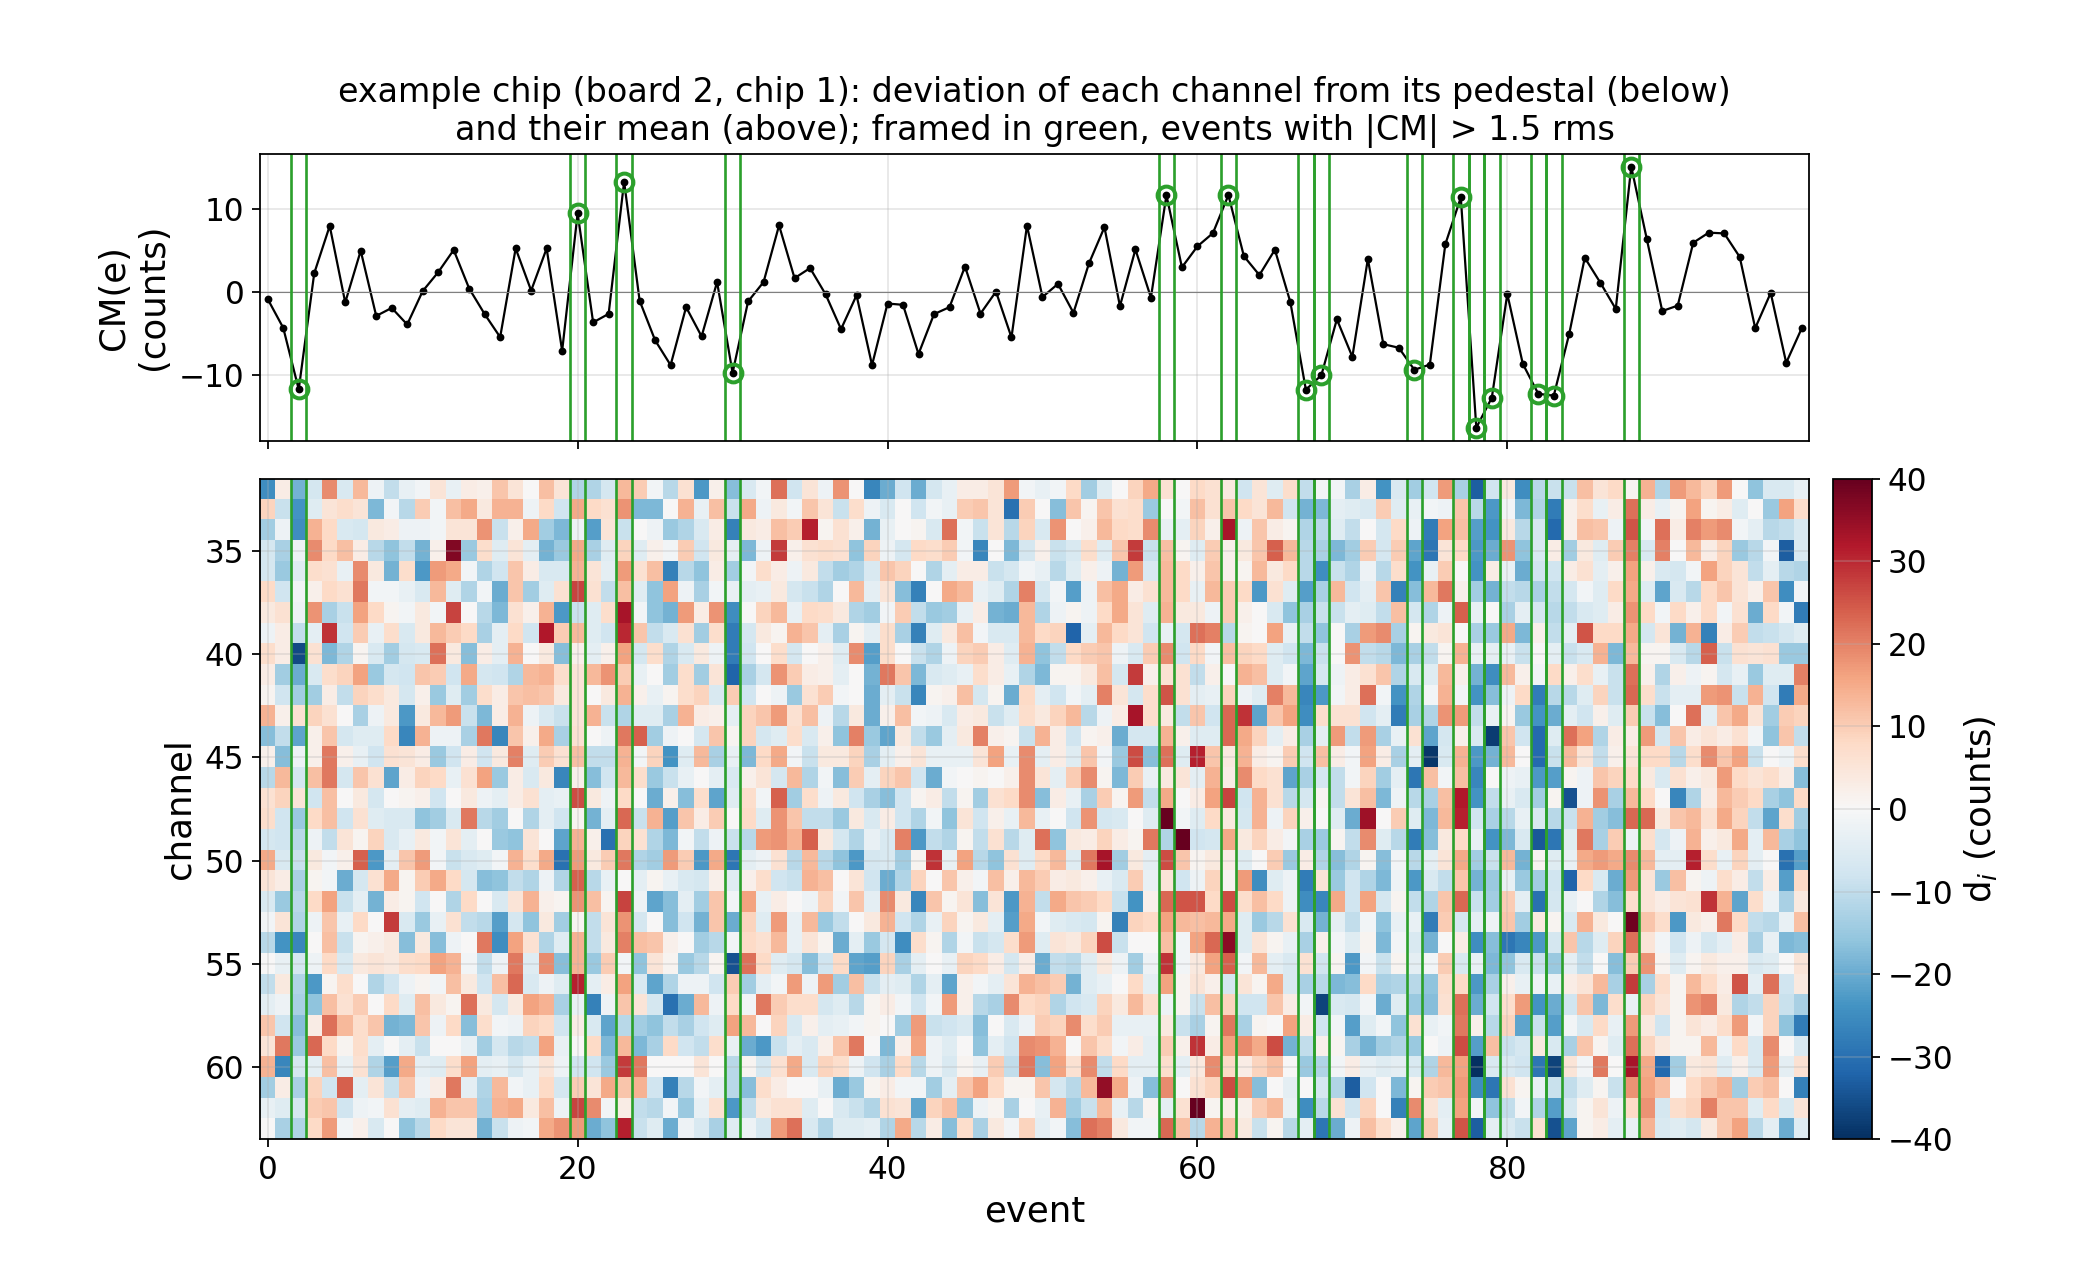
\includegraphics[width=\textwidth]{noise_steps_A.png}
\caption{Board 2, channels 32--63, run 26: deviation of each channel from its pedestal in 100
consecutive events (below), and the mean of the 32 deviations in each event (above).}
\label{fig:stepA}
\end{figure}

On the example chip $N$ is 0 in every event. On board 0, in 0.1--0.4\% of the events of most
runs, all the channels jump together by 60--230 counts (Figure~\ref{fig:stepB}); normal events
have $N \le 6$ and the jumps $N = 24$--32, so the cut separates them.

\begin{figure}[h]
\centering
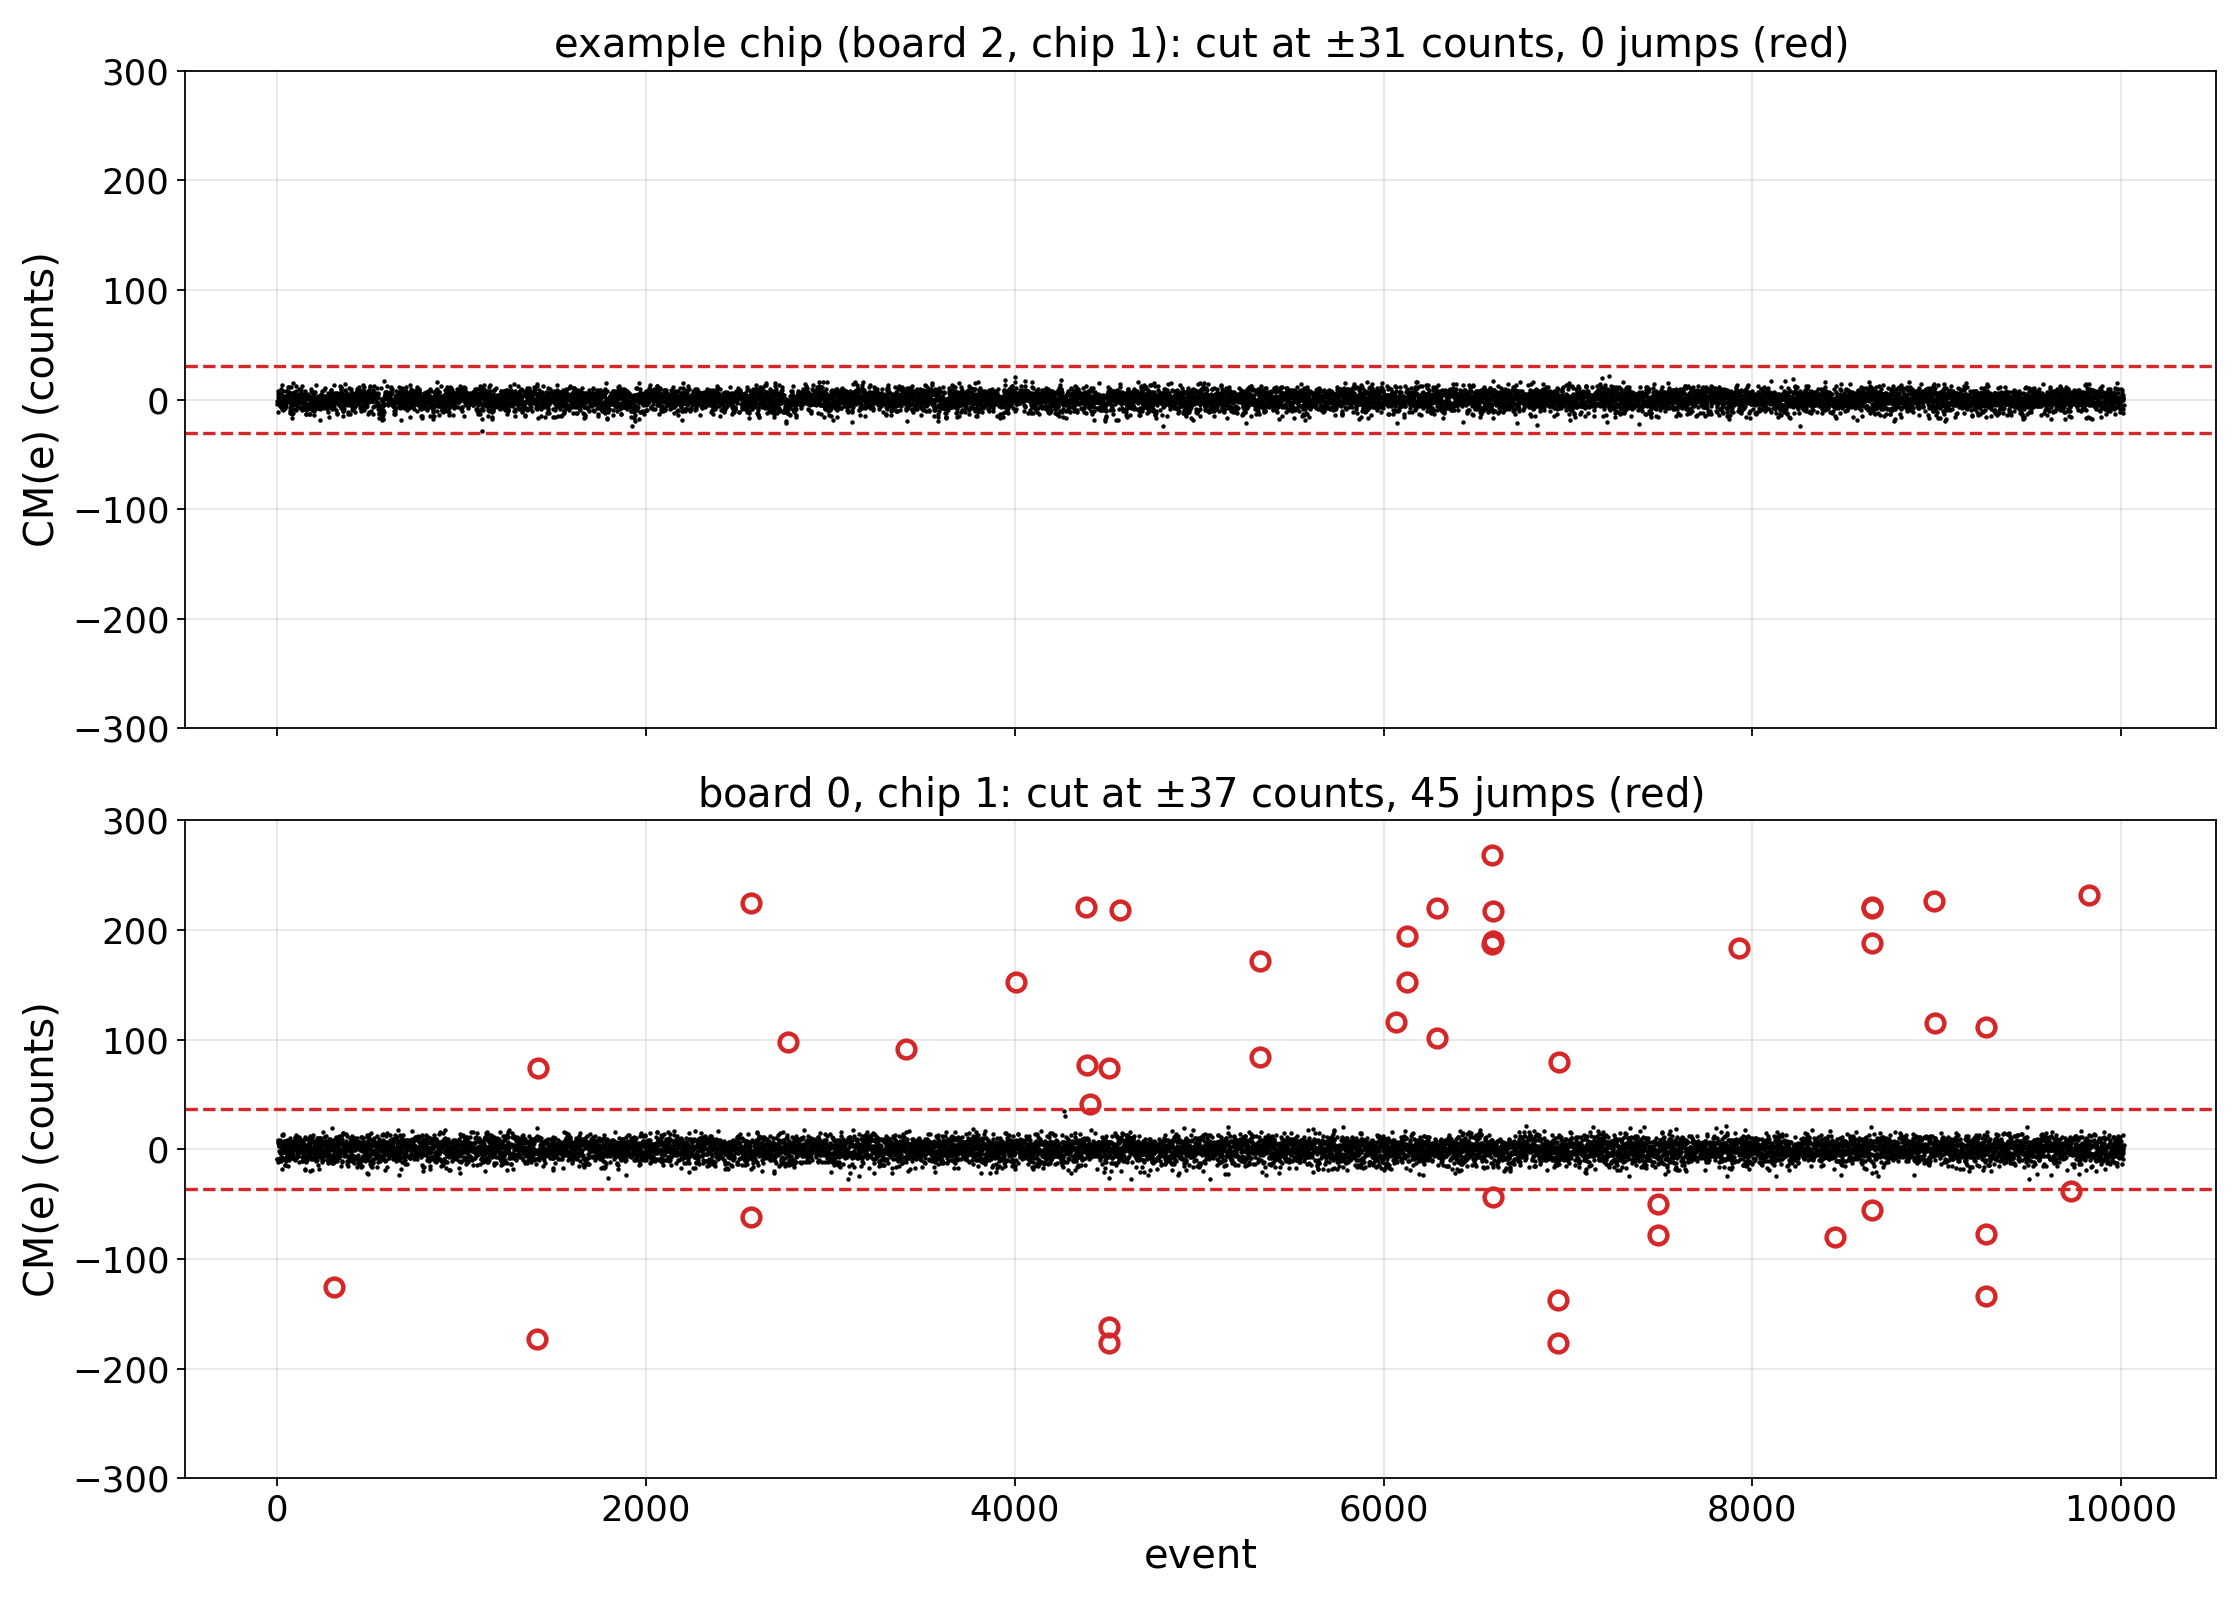
\includegraphics[width=\textwidth]{noise_steps_B.png}
\caption{Left: board 0, channels 32--63, run 26, around a jump (colour saturated at $\pm40$
counts). Right: distribution of $N(e)$ on board 0 and on the example chip, with the cut.}
\label{fig:stepB}
\end{figure}

The common mode of the example chip has an rms of 6.2 counts (Figure~\ref{fig:stepC}, left).
The slopes $b_i$ are between 0.85 and 1.2, with a median of 1.04, for all the channels of all
chips but 15, which take much less (Section~\ref{sec:sipm}); for these the assumption of a
uniform coupling holds.

\begin{figure}[h]
\centering
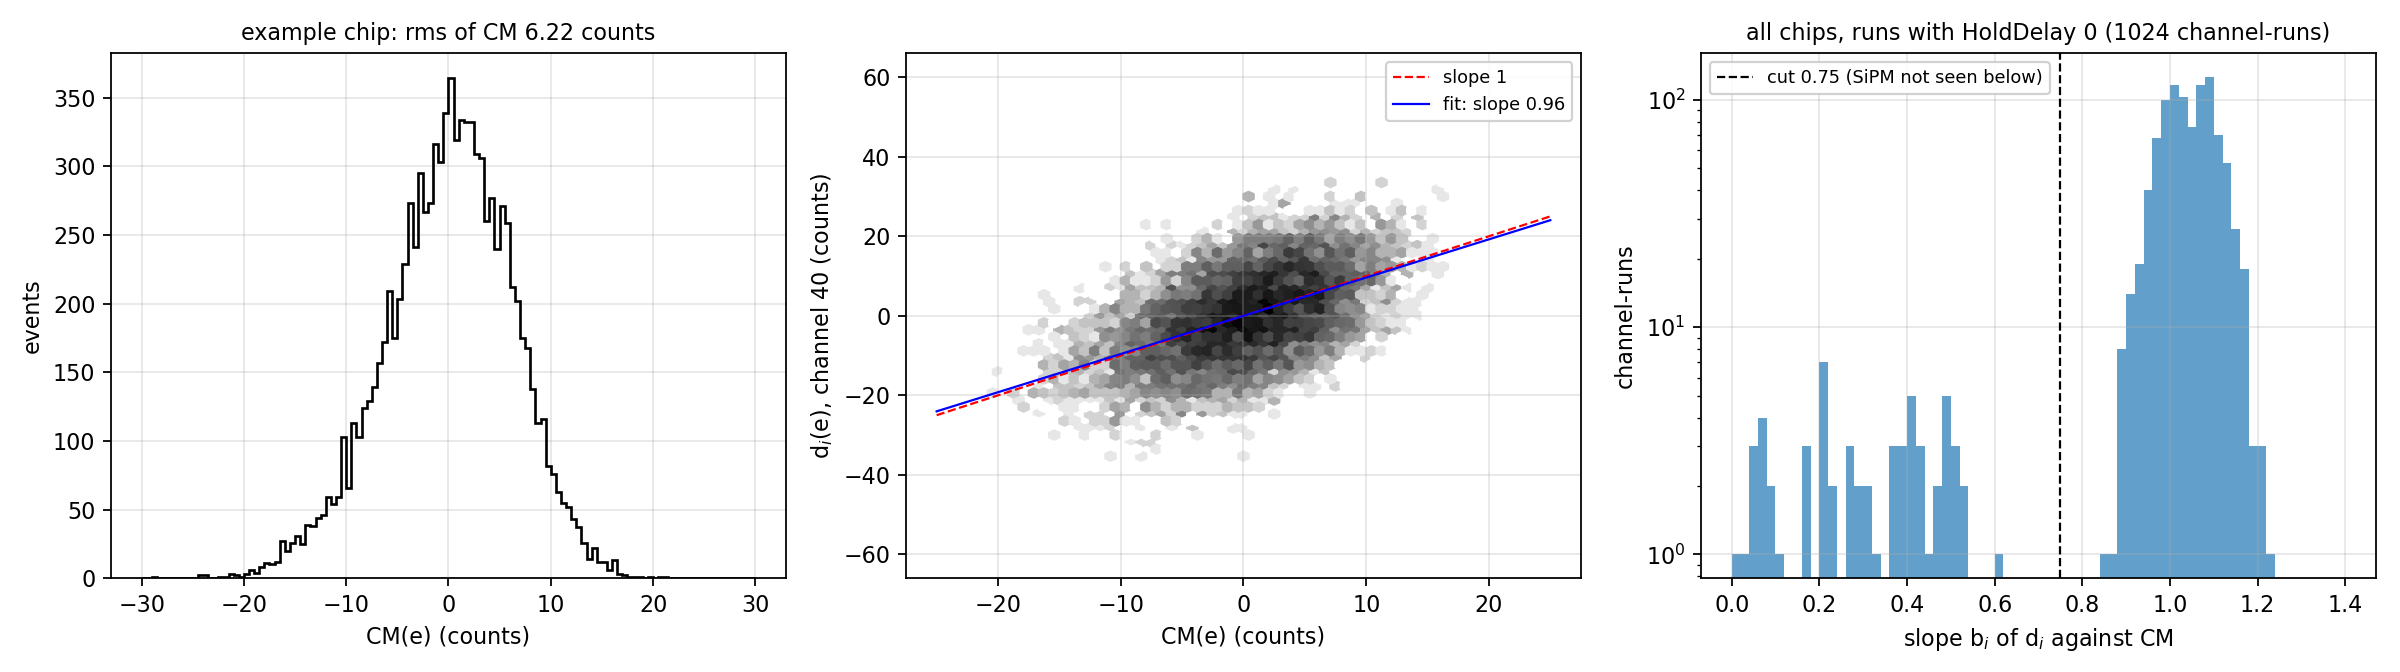
\includegraphics[width=\textwidth]{noise_steps_C.png}
\caption{Left: common mode of the example chip. Centre: deviation of channel 40 against the
common mode, with the fitted slope. Right: slopes $b_i$ of all channels in the runs with
HoldDelay 0; the channels below 0.75 do not see their SiPM.}
\label{fig:stepC}
\end{figure}

On the example chip $\sigma_\mathrm{tot} = 11.9$, $\sigma_\mathrm{coh} = 5.9$ and
$\sigma_\mathrm{inc} = 10.4$ counts, and $\sigma_\mathrm{tot}^2 = \sigma_\mathrm{coh}^2 +
\sigma_\mathrm{inc}^2$ within 0.1\%. Subtracting the common mode narrows the distribution of
the deviations from 12.0 to 10.2 counts (Figure~\ref{fig:stepD}). The common modes of the two
chips of a board are correlated by 0.6--0.85 in all boards and runs, those of different boards
by less than 0.12 (Figure~\ref{fig:stepE}): the common mode belongs to the board. In what
follows the values are medians over the chips of a run.

\begin{figure}[h]
\centering
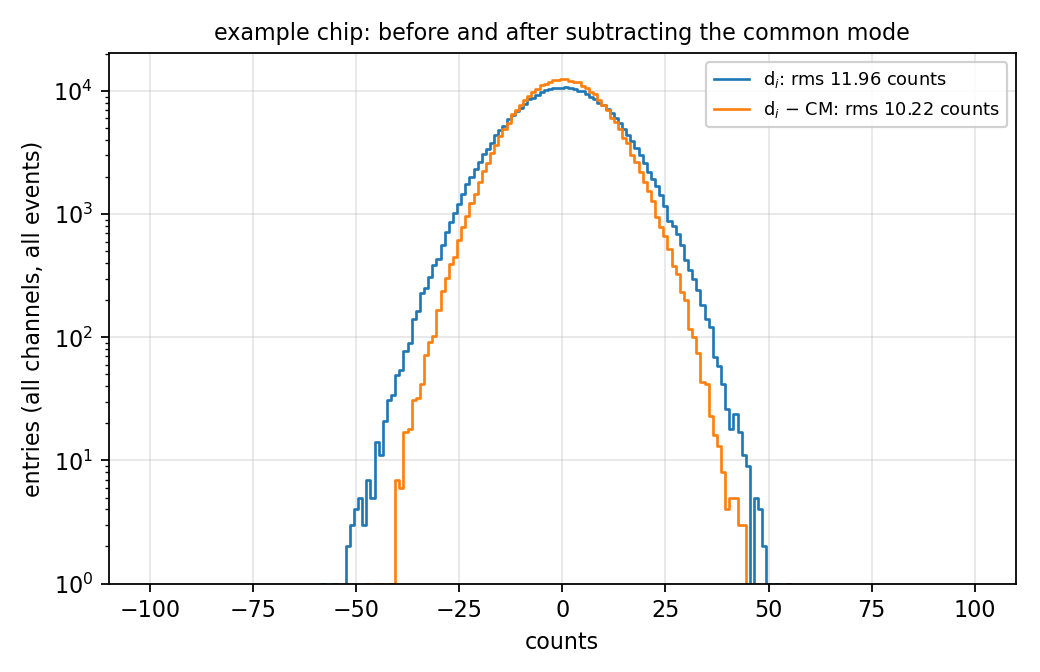
\includegraphics[width=0.55\textwidth]{noise_steps_D.png}
\caption{Example chip: deviations of all channels in all events, before and after subtracting
the common mode of each event.}
\label{fig:stepD}
\end{figure}

\begin{figure}[h]
\centering
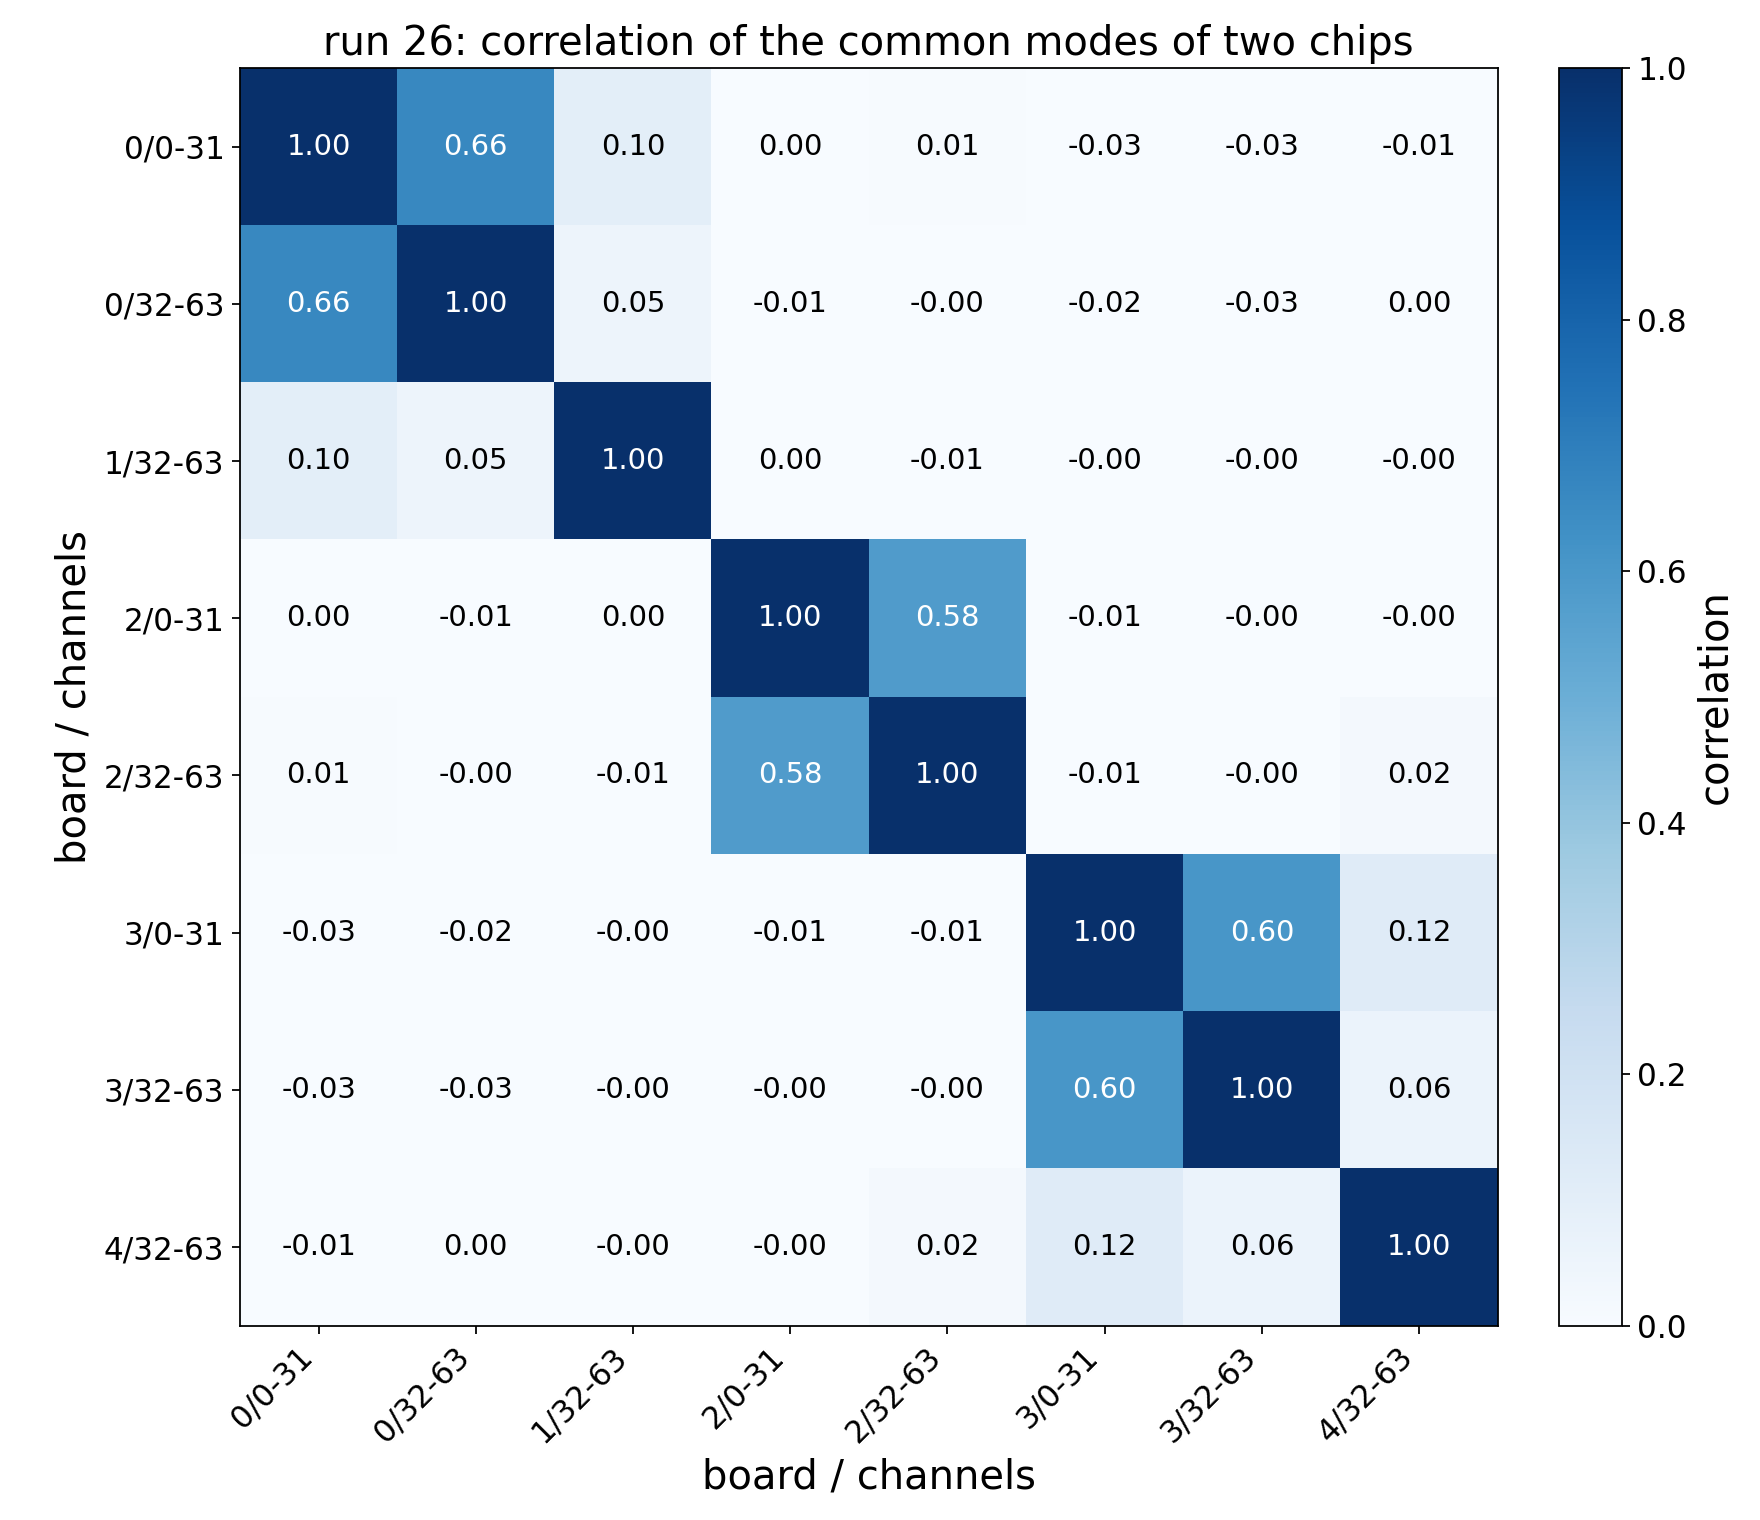
\includegraphics[width=0.8\textwidth]{noise_steps_E.png}
\caption{Common mode of chip 0 against chip 1 of board 2 (left) and of board 2 against board 3
(right), run 26.}
\label{fig:stepE}
\end{figure}

\subsection{Noise against shaping}

\begin{figure}[h]
\centering
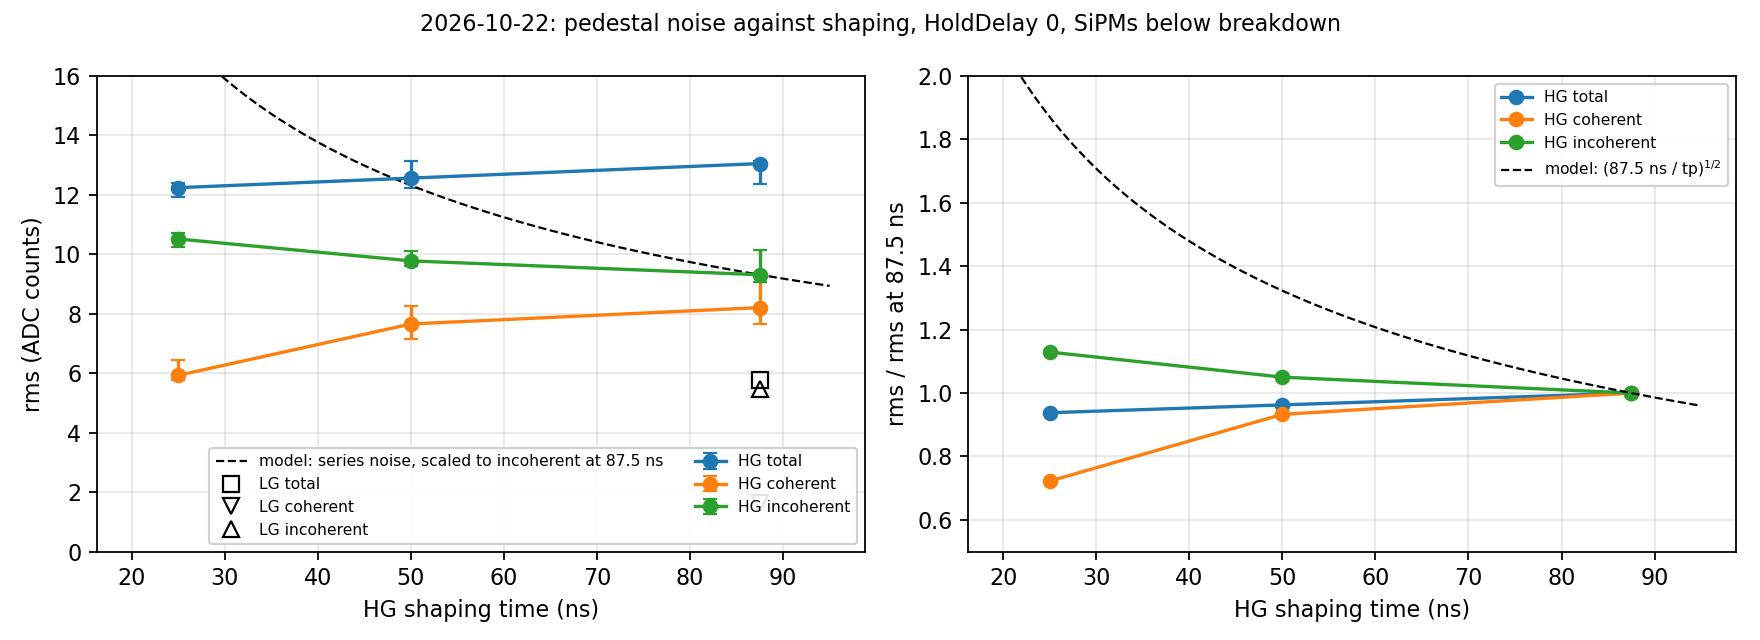
\includegraphics[width=\textwidth]{noise_vs_shaping.png}
\caption{Pedestal noise of the high gain at \texttt{HoldDelay} = 0 against the shaping time:
total, coherent and incoherent rms (median over the eight chips, bars from the lowest to the
highest chip), and the low gain at 87.5~ns. Left, in ADC counts, with the model scaled to the
incoherent noise at 87.5~ns; right, divided by the value at 87.5~ns, with the model ratio.}
\label{fig:shaping}
\end{figure}

The total noise of the high gain is 12.3, 12.6 and 13.1 counts at 25, 50 and 87.5~ns: it
barely changes, and it is slightly larger at the longest shaping, while the model predicts a
noise 1.87 times larger at 25~ns than at 87.5~ns (Figure~\ref{fig:shaping}). The two parts
behave differently. The incoherent noise, 10.5, 9.8 and 9.3 counts, does fall when the shaping
is shortened, but by 1.13 and 1.05 instead of 1.87 and 1.32. The coherent noise, 5.9, 7.7 and
8.2 counts, grows with the shaping, which is the behaviour of a noise whose power is
concentrated at low frequencies. Its share of the variance goes from a quarter at 25~ns to
40\% at 87.5~ns, so the third assumption of the model fails as well. The correlation between
the common modes of the two chips of a board is highest at the longest shaping (0.8 at
87.5~ns).

\subsection{Low gain against high gain}

At 87.5~ns, where both paths have the same shaping, the low gain has a total noise of 5.8
counts against 13.1 for the high gain, 0.45 times as much, while the model assumes the same
noise. The reduction is not the same for the two parts: the incoherent noise of the low gain
is 5.5 counts (0.59 of the high gain), its coherent noise only 1.9 (0.23).

\subsection{Pedestal against HoldDelay}

\begin{figure}[h]
\centering
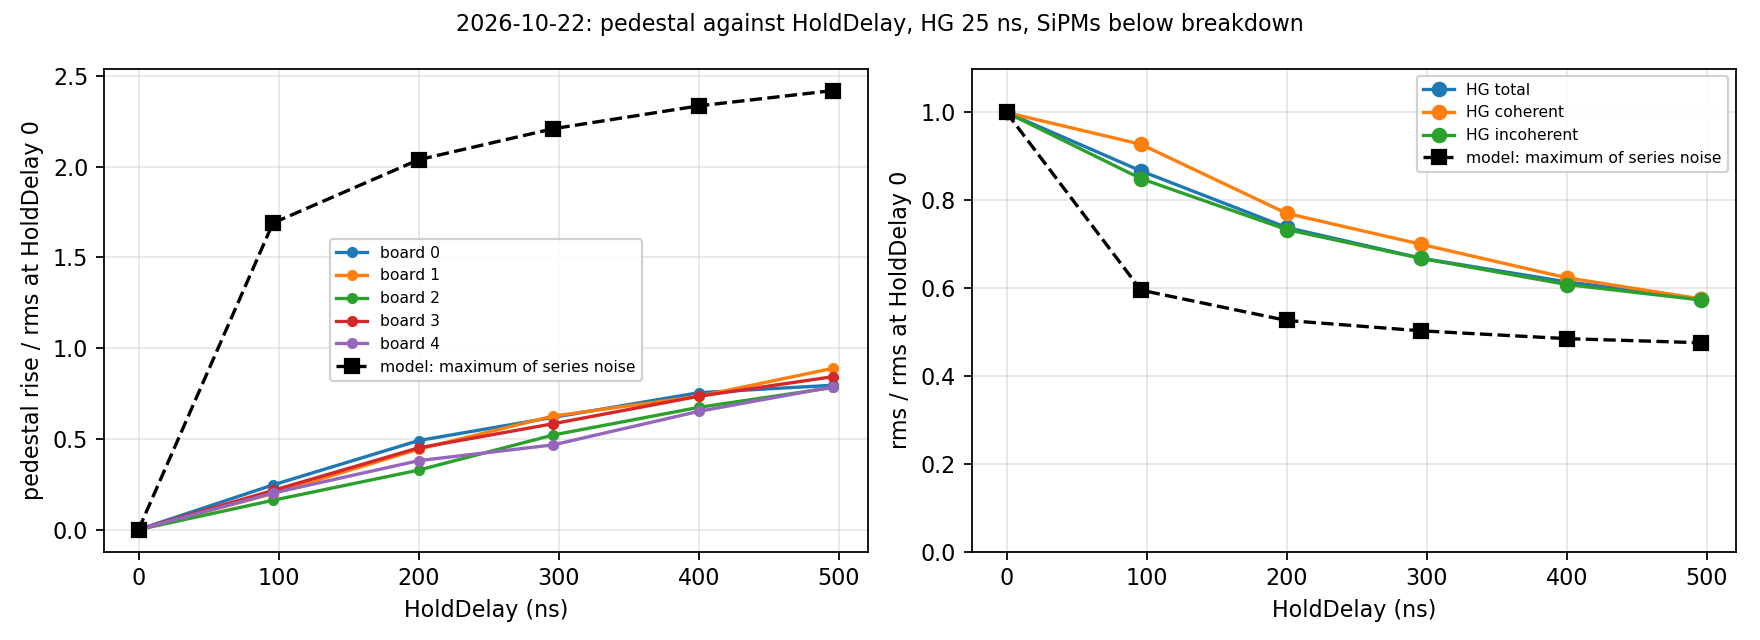
\includegraphics[width=\textwidth]{noise_vs_holddelay.png}
\caption{High gain at 25~ns against \texttt{HoldDelay}. Left, rise of the pedestal from its
value at 0~ns, in units of the total rms at 0~ns (median over the channels of each board).
Right, total, coherent and incoherent rms divided by their value at 0~ns. In black, the model:
the maximum of white noise shaped at 25~ns over a window of \texttt{HoldDelay}.}
\label{fig:hold}
\end{figure}

The pedestal rises and narrows with the window, as expected, but slowly and steadily
(Figure~\ref{fig:hold}). At 96~ns it has risen by 0.2 rms against 1.7 in the model, at 296~ns
by 0.5--0.6 against 2.2, and at 496~ns by 0.8--0.9 against 2.4, and it has not yet stopped
rising. The width falls to 0.87 of its initial value at 96~ns and to 0.58 at 496~ns, where the
model reaches 0.6 already at 96~ns and stays at about 0.5. The coherent and incoherent parts
narrow in the same way. The data therefore behave as if the noise kept its value for a few
hundred nanoseconds, much longer than the shaping time, so that a longer window adds new
fluctuations only slowly.

\subsection{The common mode enters through the SiPM}
\label{sec:sipm}

Fifteen channels take much less common mode than the others, with slopes $b_i$ of 0.02--0.6
in all runs against more than 0.85 for every other channel (Figure~\ref{fig:slopes}). On
board 0 they are channels 15, 55, 57, 59, 61 and 63, exactly the six channels that showed no
avalanches in the threshold scans taken on 21 October with the SiPMs above breakdown, whose
SiPM is connected but whose signal is lost in a bad contact or in the connector. The other
nine are on boards 1, 3 and 4, where no threshold scan has been taken yet. A channel that does
not see its SiPM does not receive the common mode, so the common mode reaches the
preamplifiers through the SiPMs. The pedestal rms alone does not separate these channels: a
SiPM at the input raises the noise of its preamplifier, but at 87.5~ns the six channels sit at
0.82--0.87 of the median rms of their board and other channels at 0.81--0.89. The slope is
therefore also a test, from a pedestal run, of whether each channel sees its SiPM.

\begin{figure}[h]
\centering
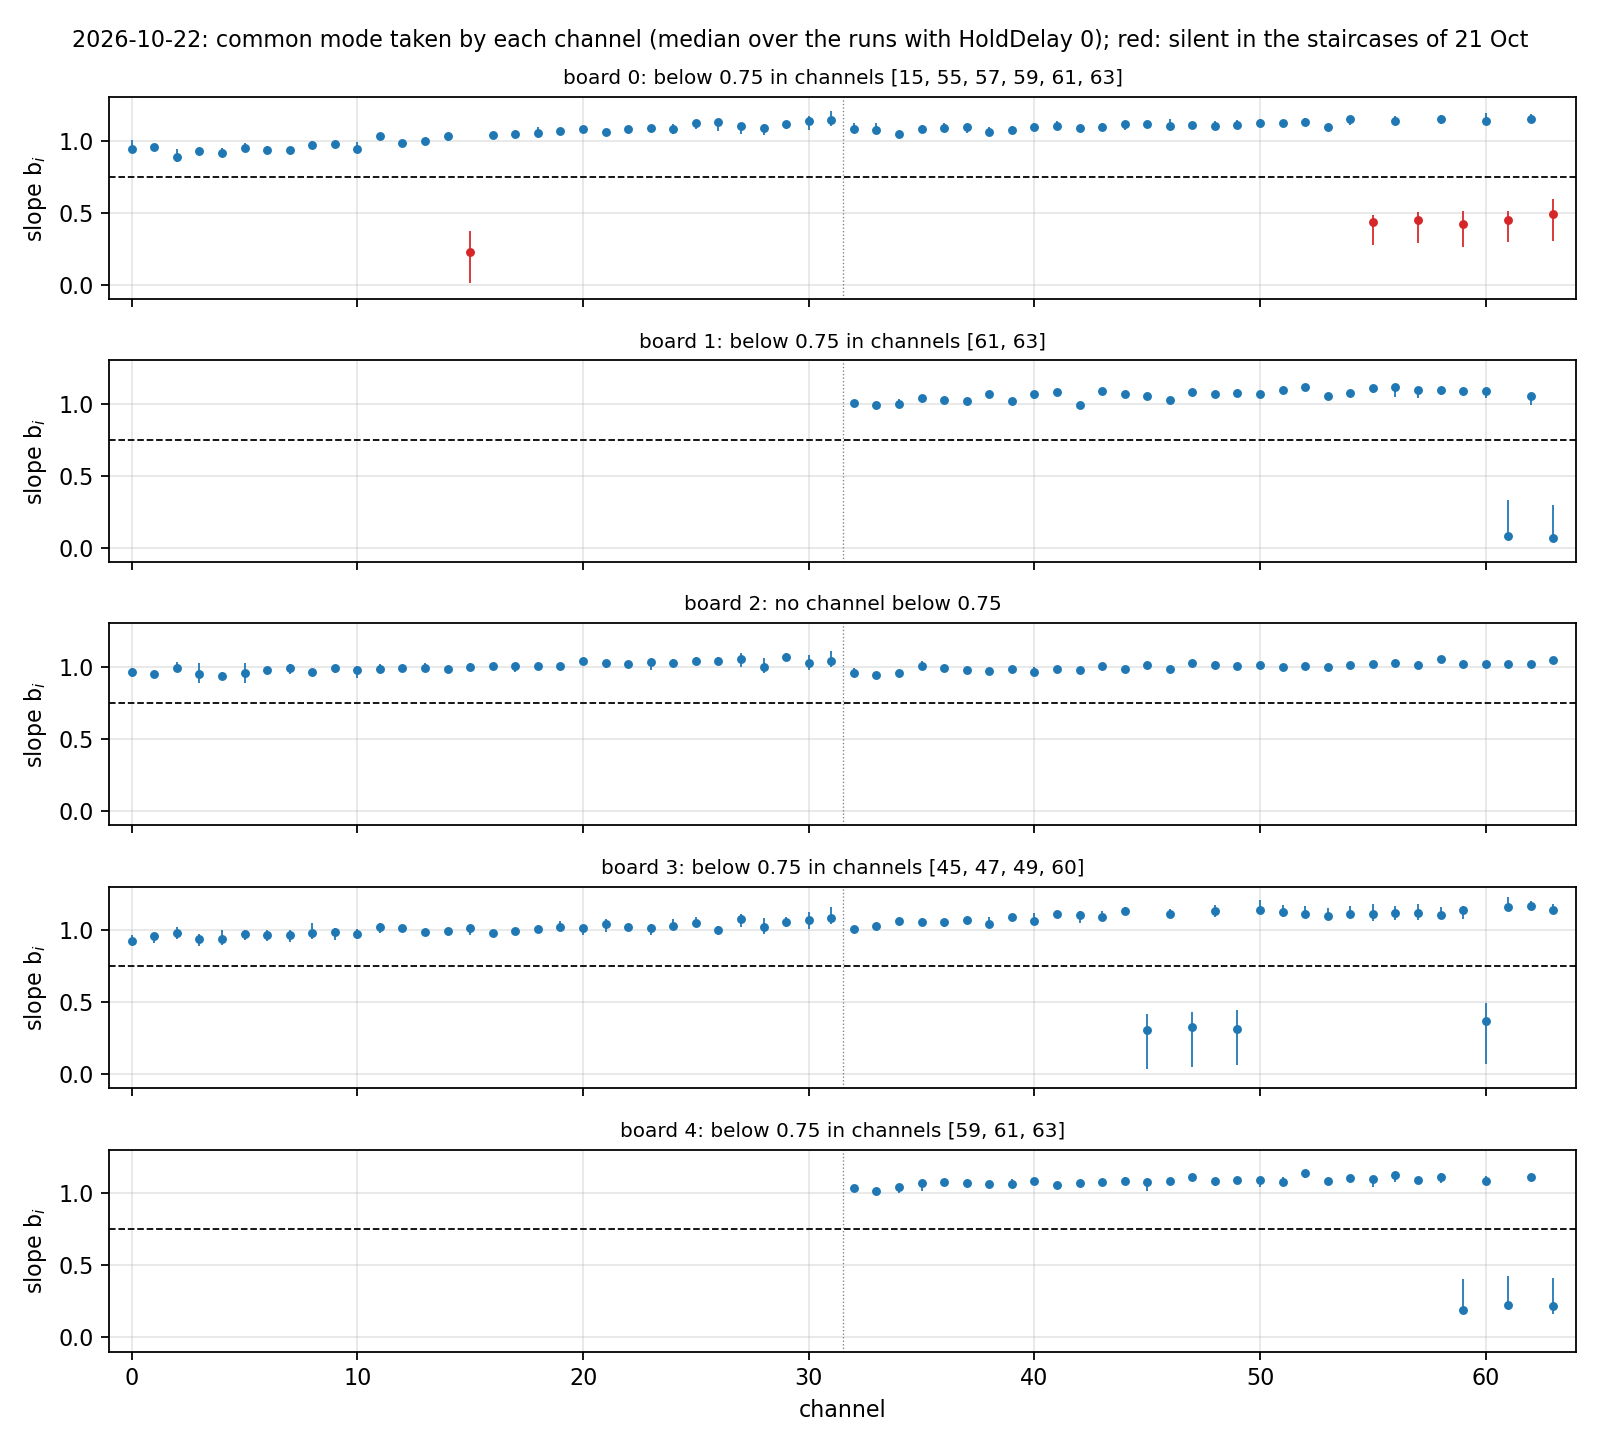
\includegraphics[width=\textwidth]{bench_slopes.png}
\caption{Slope of each channel against the common mode of its chip, median over the runs with
HoldDelay 0 (bars from the lowest to the highest run), with a cut at 0.75. In red, the six
channels of board 0 without avalanches in the threshold scans.}
\label{fig:slopes}
\end{figure}

\section{Hypotheses}

\begin{enumerate}
\item \textbf{A low-frequency noise dominates.} A mixture in which the $1/f$ or parallel
  components dominate gives a noise nearly independent of the shaping, and a noise with long
  correlation times explains the slow rise of the pedestal with the window. The two
  observations would then have one cause.
\item \textbf{The coherent noise comes from the bias of the SiPMs.} The HV module of each board
  biases its 64 SiPMs through a common line; below breakdown each SiPM is a capacitor that
  couples any ripple of that line to the input of its preamplifier. This gives a noise common
  to the board, uncorrelated between boards and concentrated at low frequencies, as observed,
  and it explains why channels without their SiPM do not receive the common mode
  (Section~\ref{sec:sipm}); the reference voltages or the ground of the board would reach
  every channel, connected or not. A pick-up on the cables or adapter boards between the
  SiPMs and the board would also enter through the SiPMs and is not excluded.
\item \textbf{The peak detector is not ideal.} If the peak detector follows the signal with a
  finite speed, or loses part of the held value during the window, it acts as a further
  filter and the rise with the window is slower than for an ideal maximum. This would affect
  the response to real pulses as well.
\item \textbf{The low gain has its own noise.} If the coherent part enters before the
  preamplifiers, it is scaled by the ratio of their gains, while the incoherent part, partly
  their own, is reduced less, as observed. A model with the same noise in counts in both gains
  is then too simple.
\end{enumerate}

\section{What is needed}

\begin{enumerate}
\item \textbf{The gain in counts per pe}, at 25, 50 and 87.5~ns, to express the noise in
  photoelectrons and compare with the 0.06--0.11~pe of the model. It comes from the
  hold-delay scans with the SiPMs at 5~V of overvoltage (bench note 2), on the plateau where
  the single-pe peaks are resolved, and from the calibration with the periodic trigger
  (bench note 3).
\item \textbf{The response of the peak detector to a known pulse}, from the same hold-delay
  scans: the delay after the trigger at which the stored amplitude reaches its plateau,
  compared with the 31, 58 and 90~ns of the model (plus the latency of the board), and whether
  the plateau stays flat at long delays. This tests the third hypothesis and shows that the
  shaping time actually changes.
\item \textbf{Threshold scans of the five boards} (bench note 2), to test the prediction of
  Section~\ref{sec:sipm} for the nine channels of boards 1, 3 and 4.
\item \textbf{A pedestal run with the HV off}, at 25 and 87.5~ns. The SiPMs stay connected,
  so a pick-up on the cables would remain, while a ripple of the bias line would disappear
  with the coherent noise. This decides the origin of the coherent noise (second
  hypothesis).
\item \textbf{The analog probe of the slow shaper on the oscilloscope}, with the SiPMs below
  breakdown: the noise waveform gives its correlation time and its spectrum directly, and
  decides between the first and the third hypotheses.
\item \textbf{A fit of the model to both data sets}, on our side: series, parallel and $1/f$
  components, plus a coherent component per board, adjusted to the noise against shaping and
  to the pedestal against the window at the same time.
\end{enumerate}
\noindent The first three come from the next bench session (bench note 2); the fourth and
fifth are short additions to be scheduled after it.

\section{Status for the model}

Nothing is yet stable enough to replace the noise model of the simulation. What the
measurements already establish, in ADC counts, is that the noise of a channel has a coherent
part shared by the 64 channels of a board, entering through the SiPMs, of 25--40\% of the
variance; that neither part follows the $t_p^{-1/2}$ scaling; that the low gain has 0.45 times
the noise of the high gain; and that the noise varies over hundreds of nanoseconds. For the
sum of the 64 channels, which gives the energy, the coherent part matters most: the incoherent
noise adds in quadrature and grows as $\sqrt{64} = 8$ times that of one channel, while the
coherent noise adds almost linearly. With the numbers of the high gain at 25~ns, about 85
counts come from the incoherent noise and about 350 from the coherent one (with the measured
correlation of 0.6--0.85 between the two chips of a board). The model will need a correlated
component per board and a dependence on the shaping and on the window taken from the data.

To pass a result to the model, three things are missing: the gain, to express the noise in
photoelectrons; the origin of the coherent noise, since a ripple of the bias may change with
the HV module or be filtered, while a pick-up depends on the cabling, which will change with
the new adapter board; and the behaviour of the peak detector, which decides whether the slow
rise with the window is a property of the noise or of the chip.

\section*{Implementation}

The decoded runs are read by \path{fullsim_analysis/scripts/bench/inspect_run.jl}, which writes
the pedestal, rms and robust width of each channel (\path{channels.csv}), and
\path{fullsim_analysis/scripts/bench/noise_components.jl}, which writes the total, coherent and
incoherent noise of each chip (\path{noise_components.csv}), the correlation of the common
modes between chips (\path{common_mode.csv}) and the slope of each channel
(\path{channel_slopes.csv}), all in \path{fullsim_analysis/results/bench/2026-10-22/}. The
method of Section~\ref{sec:cm} is implemented once, in \path{fullsim_analysis/lib/chip_noise.jl},
so that bench and simulated pedestal runs are analysed by the same code;
\path{noise_steps.jl} writes the data of Figures~\ref{fig:stepA}--\ref{fig:stepE}. The figures
are produced by \path{fullsim_analysis/plots/noise_steps.py}, \path{bench_noise.py}
(Figure~\ref{fig:slopes}) and \path{model_data_noise.py}, which also computes the model curves
(white noise through CR-RC$^2$ on a 1~ns grid, maximum over the window, 20\,000 windows).

\end{document}
